\documentclass[a4]{jsarticle}
\usepackage[dvipdfmx]{graphicx}
\usepackage[labelsep=period]{caption}
\usepackage{listings, jlisting}
\usepackage[]{amsmath}
\usepackage{here}
\usepackage[top=25truemm, bottom=25truemm, left=25truemm, right=25truemm]{geometry}
\usepackage[]{url}

\lstset {
	language={Python},
	basicstyle={\tt},
	identifierstyle={\tt},
	commentstyle={\bf},
	keywordstyle={\bf},
	ndkeywordstyle={},
	stringstyle={\ttfamily},
	frame={single},
	framesep=5pt,
	breaklines=true,
	numbers=left,
	numberstyle={\ttfamily},
	tabsize=4
}

\title{}
\author{開放環境科学専攻 82119176 冨田寿子}
\date{}

\begin{document}
\maketitle

\section{カバーストーリー}
迷路状の入り組んだ空間の右端にピンクのドロップが居て,赤い花を欲しがっている.
左端には青いドロップがいて,ピンクのドロップのために花を持っていくことを目的と
している.
しかし,花畑の近くにはオレンジのドロップが花を守るように見張っている.
青いドロップは一度花の中に立ち入り,オレンジのドロップは鑑賞は許してくれた.
しかし,青いドロップは赤い花を取るために青い花を踏んだため,オレンジのドロップは
怒ってしまった.
青いドロップは逃げ出し,オレンジのドロップは見張りの範囲を広げた.
青いドロップは別のルートから花を取ろうと様子を伺い,タイミングを見計らって花畑
に入る.
青いドロップは手前の青い花と目的の赤い花を取り,花畑を出る.
オレンジのドロップは,花を持った青いドロップが花畑から出てくるのを見つけ,
追いかける.
青いドロップは逃げる最中,細い道に青い花を置いた.
オレンジのドロップは花を踏めないため先に進めず,追いかけるのを諦め,花畑に戻る.
青いドロップはピンクのドロップのもとへ赤い花を持って行き,花をつけてあげる.

\section{作成方法}
PythonでOpenCVを動かし,背景画像にドロップや花の画像を上に重ね,1コマごとに位置を
変えることで動画を作成した.
また,3つのドロップが同時に動くため,1つの関数内に3つのドロップそれぞれのx,y座標
方向を引数に取り,同時に異なった動きができるようにした.
\begin{lstlisting}[caption=3つのドロップの位置]
	# prt : blue drop
	# px, py, dir_p : blue_drop's position and direction
	# enemy : orange drop
	# ex, ey, dir_e : orange drop's position and direction
	# friend : pink_drop
	# fx, fy, dir_f : pink drop's position and direction
	# bg : back ground, flowers' position is different
	def ahead(save, prt, px, py, dir_p, enemy, ex, ey, dir_e, friend, fx, fy, dir_f, bg):
		image = CvOverlayImage.overlay(bg, rotate(prt, dir_p), (px, py))
		image = CvOverlayImage.overlay(image, rotate(enemy, dir_e), (ex, ey))
		save_image(save, image, prt, px, py, enemy, ex, ey, friend, fx, fy)
\end{lstlisting}
ピンクのドロップは,青いドロップを待っているため,常に青いドロップの方向を向くように
逐次2つの位置情報から方向を計算するようにした.

\begin{lstlisting}[caption=ピンクのドロップの方向計算]
	# px, py : blue drop's position
	# fx, fy : pink drop's position
	diff_x = px - fx + 1
	diff_y = py - fy
	if diff_y < 0 and diff_x >= 0:
	direction = - math.degrees(math.atan(diff_y / diff_x))
	elif diff_y < 0 and diff_x < 0:
	direction = 180 - math.degrees(math.atan(diff_y / diff_x))
	elif diff_y > 0 and diff_x < 0:
	direction = 180 - math.degrees(math.atan(diff_y / diff_x))
	elif diff_y > 0 and diff_x >= 0:
	direction = - math.degrees(math.atan(diff_y / diff_x))
	elif diff_y == 0 and px > fx:
        direction = 0
	elif diff_y == 0 and px < fx:
        direction = 180
	elif diff_x == 0 and py > fy:
        direction = 90
	elif diff_x == 0 and py < fy:
        direction = -90
	\end{lstlisting}
また,ドロップが1歩1歩進んでいる様子を表すため,進行方向に対して$\pm 30$度
ずつ左右にドロップの先端を振りながら進むようにした.

\begin{figure}[htbp]
	\begin{minipage}[t]{0.3\hsize}
		\begin{center}
			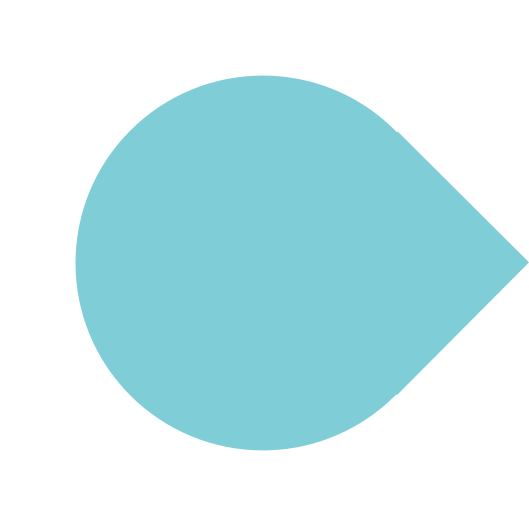
\includegraphics[scale=0.2]{../imgs2/drop_blue.png}
			\caption{青いドロップ}
			\label{fig:blue_drop}
		\end{center}
	\end{minipage}
	\begin{minipage}[t]{0.3\hsize}
		\begin{center}
			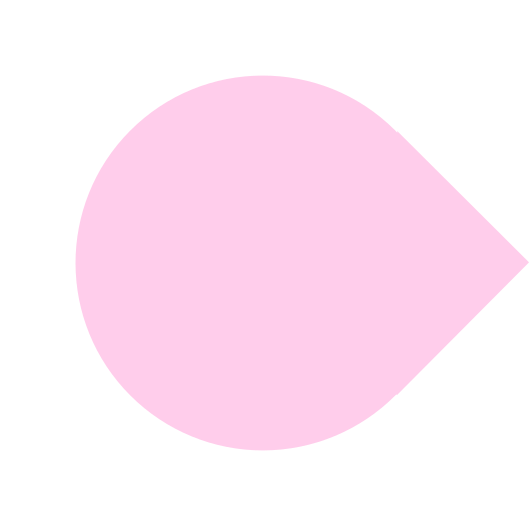
\includegraphics[scale=0.2]{../imgs2/drop_pink.png}
			\caption{ピンクのドロップ}
			\label{fig:pink_drop}
		\end{center}
	\end{minipage}
	\begin{minipage}[t]{0.3\hsize}
		\begin{center}
			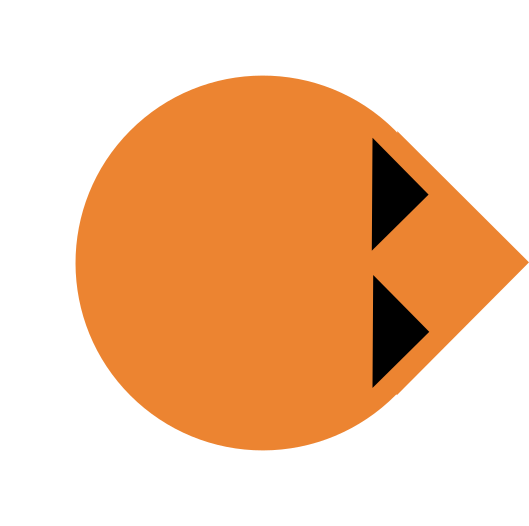
\includegraphics[scale=0.2]{../imgs2/enemy.png}
			\caption{オレンジのドロップ}
			\label{fig:pink_drop}
		\end{center}
	\end{minipage}
\end{figure}
\begin{figure}[htbp]
	\begin{minipage}[t]{0.5\hsize}
		\begin{center}
			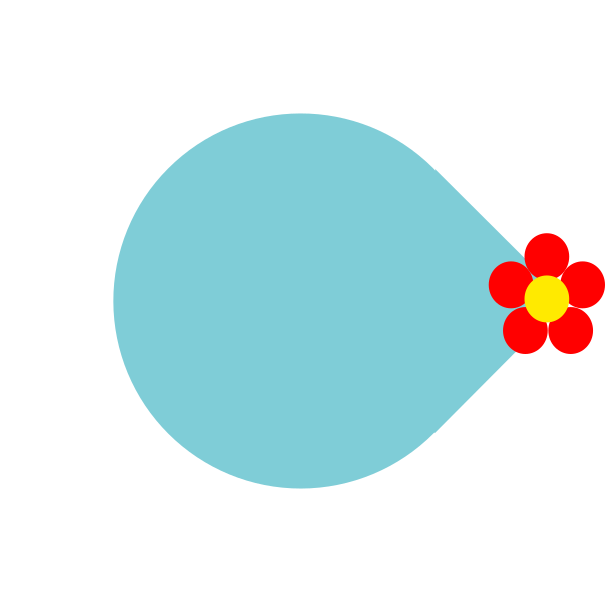
\includegraphics[scale=0.2]{../imgs2/drop_blue_flower.png}
			\caption{花を持った青いドロップ}
			\label{fig:blue_drop_flower}
		\end{center}
	\end{minipage}
	\begin{minipage}[t]{0.5\hsize}
		\begin{center}
			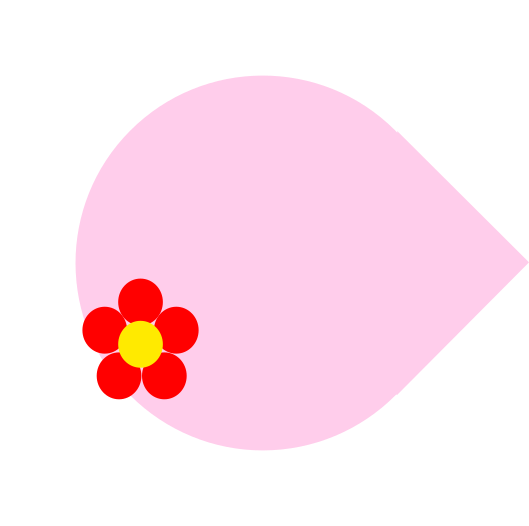
\includegraphics[scale=0.2]{../imgs2/drop_pink_flower.png}
			\caption{花をつけたピンクのドロップ}
			\label{fig:pink_drop_flower}
		\end{center}
	\end{minipage}
\end{figure}
\begin{figure}[htbp]
	\begin{minipage}[t]{0.3\hsize}
		\begin{center}
			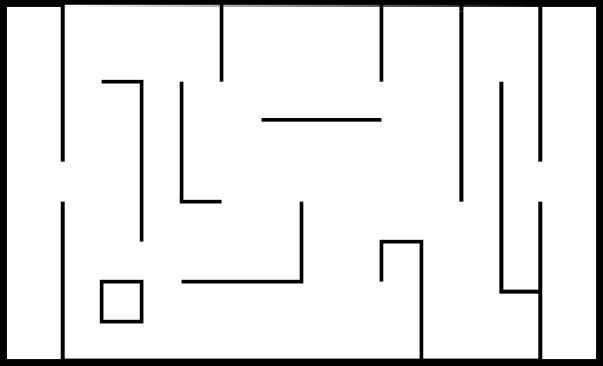
\includegraphics[scale=0.4]{../imgs2/bg.png}
			\caption{背景}
			\label{fig:bg}
		\end{center}
	\end{minipage}
	\begin{minipage}[t]{0.3\hsize}
		\begin{center}
			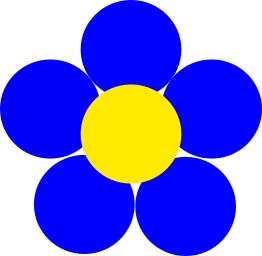
\includegraphics[scale=0.2]{../imgs2/flower_blue.png}
			\caption{青い花}
			\label{fig:flower_blue}
		\end{center}
	\end{minipage}
	\begin{minipage}[t]{0.3\hsize}
		\begin{center}
			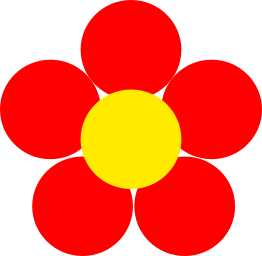
\includegraphics[scale=0.2]{../imgs2/flower_red.png}
			\caption{赤い花}
			\label{fig:flower_red}
		\end{center}
	\end{minipage}
\end{figure}

\section{cohenの定義に基づく意図のある行動}
\subsection{定義8.1}
青いドロップxは,赤いドロップに赤い花を渡すという約束のもとで花畑から赤い花を取る
というサブゴールを持っている.
\begin{align*}
	&(P-R-GOAL \, x \, p \, q) \\
	&= (GOAL \, x (LATER \, x \, PICK(x \, red\_flower))) \land (BEL \, x \, \neg PICK(x \, red\_flower)) \\
	&\land (BEFORE [(BEL \, x \, PICK(x \, red\_flower)) \lor (BEL \, x \, □ \neg \, PICK(x \, red\_flower)) \lor \\
	&(BEL \, x \, (LATER \, x \, \neg GIVE(x \, red\_flower)))] \neg (GOAL \, x \, (LATER \, PICK(x \, red\_flower))))
\end{align*}

オレンジのドロップxは,花を守るという強い決意のもとで花を取った青いドロップを
追いかけている.
\begin{align*}
	&(P-R-GOAL \, x \, p \, q) \\
	&= (GOAL \, x (LATER \, x \, CHASE(x \, blue\_drop))) \land (BEL \, x \, \neg CHASE(x \, blue\_drop)) \\
	&\land (BEFORE [(BEL \, x \, CHASE(x \, blue\_drop)) \lor (BEL \, x \, □ \neg \, CHASE(x \, blue\_drop)) \lor \\
	&(BEL \, x \, (LATER \, x \, \neg SAVE(x \, flowers)))] \neg (GOAL \, x \, (LATER \, CHASE(x \, blue\_drop))))
\end{align*}

\subsection{定義8.2}
青いドロップxは,赤い花をピンクのドロップに渡すという約束のもとで花を取るという
アクションをする.
\begin{align*}
	&(INTEND1 \, x \, p \, q) = \\
	&(P-R-GOAL \, x \, [DONE \, x (BEL \, x (HAPPENS \, x \, PICK(x \, blue\_flower) \, ; \\
	&PICK(x \, red\_flower) \, ; \, HAVE(x \, flowers)?)?) \\
	&PICK(x \, blue\_flower) \, ; \, PICK(x \, red\_flower) \, ; \, HAVE(x \, flowers)?] \\
	&GIVE(x \, red\_flower))
\end{align*}

オレンジのドロップxは,すべての花を守るという決意のもとで花畑の周辺を見回り,花を持った
青いドロップを見つけると捕まえようとするアクションをする.
\begin{align*}
	&(INTEND1 \, x \, p \, q) = \\
	&(P-R-GOAL \, x \, [DONE \, x (BEL \, x (HAPPENS \, x \, LOOK\_AROUND(x \, flowers) \, ; \\
	&LOOK(x \, flower\_thief) \, ; \, CHASE(x \, flower\_thief) \, ; \, SAVE(x \, flowers)?)? \\
	&LOOK\_AROUND(x \, flowers) \, ; \, LOOK(x \, flower\_thief) \, ; \, \\
	&CHASE(x \, flower\_thief) \, ; \, CHASE(x \, flower\_thief) \, ; \, SAVE(x \, flowers)] \\
	&SAVE(x \, all\_flowers))
\end{align*}

\subsection{定義8.3}
青いドロップxは,赤い花をピンクのドロップに渡すという約束のもとで,赤い花を取る.
\begin{align*}
	&(INTEND2 \, x \, p \, q) = \\
	&(P-R-GOAL \, x \, PICK(x \, red\_flower) (DONE \, x [(BEL \, x \, PICK(x \, red\_flower) \\
	&(HAPPENS \, x \, PICK(x \, red\_flower) \, ; \, HAVE(x \, red\_flower)?)) \\
	&\land \neg (GOAL \, x \, \neg(HAPPENS \, x \, PICK\_ACCIDENTALY(x \, red\_flower) \, ; \\
	&HAVE(x \, red\_flower)?))]? ; PICK(x \, red\_flower) \, ; \, HAVE(x \, red\_flower)?) \\
	&GIVE(x \, red\_flower))
\end{align*}

\subsection{定義6.1}
青いドロップxは,オレンジのドロップから逃れるため,青い花を取るというアクションを
起こす.
しかし,この行為に約束や強い意思はないため,定義8.2にはならない.
\begin{align*}
	&(INTEND1 \, x \, a) = \\
	&(P-GOAL \, x [DONE \, x (BEL \, x (HAPPENS \, PICK(x \, blue\_flower))? \, ; \, \\
	&PICK(x \, blue\_flower))])
\end{align*}

\subsection{定義6.2}
青いドロップxはオレンジのドロップの行く手を阻むために青い花を道に置く.
この行動も,定義8.3のqにあたる約束や強い意思はない.
\begin{align*}
	&(INTEND2 \, x \, a) = \\
	&(P-GOAL \, x \, PICK(x \, blue\_flower) (DONE \, x [(BEL \, x \, PICK(x \, blue\_flower) \\
	&(HAPPENS \, x \, PICK(x \, blue\_flower) \, ; \, PREVENT(x \, CATCH(orange\_drop \, blue\_drop))?)) \\
	&\land \neg(GOAL \, x \, \neg(HAPPENS \, x \, VANISH(x \, orange\_drop) \, ; \,\\
	&PREVENT(x \, CATCH(orange\_drop \, blue\_drop))?))] \, ; PICK(x \, blue\_flower) \, ; \\
	&PREVENT(x \, CATCH(orange\_drop \, blue\_drop))?))
\end{align*}

\section{映像中の定義に基づく行動の詳細}
\subsection{定義8.1}
青いドロップは,ピンクのドロップに赤い花を渡すことを目的としているため,ピンクの
ドロップが赤い花を待っている限り,青いドロップは目的を果たそうとする.
ピンクのドロップは赤い花を持っておらず,青いドロップもそれを信じている.
したがって,サブゴールpは青いドロップが赤い花を得ることで,スーパーゴールqは
ピンクのドロップに赤い花を渡すことである.

オレンジのドロップは,花を守るというスーパーゴールqがある.
そのため,花が存在する限りオレンジのドロップは花を守るための行動をする.
オレンジのドロップは,花がなくなる未来を想定しており,それを阻止するために花を
取った青いドロップを捕まえるというサブゴールを設定している.

\subsection{定義8.2}
青いドロップが赤い花を取るというアクションは意図を持って行っている.
その最中,オレンジのドロップを避けながら赤い花のもとへ進んでいるため,偶然
花のある場所を通りかかったわけではない.
また,定義8.2のqにあたる約束は,ピンクのドロップに赤い花を渡すことである.

オレンジのドロップは,すべての花を守るという強い決意qのもとで,花畑の周辺を見回るという
アクションを行っている.
また,花を取った青いドロップを見つけると,青いドロップを捕まえるというアクション
を起こすことで花を守るというサブゴールが達成できると信じている.
青いドロップを逃し,すべての花を守れないとなった時点で青いドロップを追いかけるという
アクションをやめている.

\subsection{定義8.3}
青いドロップは,赤い花をピンクのドロップに渡すという約束qのもとで,赤い花を
取るというゴールpをする.
また,花畑に行くというアクションを起こすことで赤い花を取るというゴールを果たせる
と信じており,道中偶然に赤い花が落ちていることは想定していない.
さらに,一度オレンジのドロップに阻まれても再度赤い花を取るよう行動しており,
簡単にはサブゴールの達成を諦めていない.

\subsection{定義6.1}
青いドロップは,オレンジのドロップから逃れるため,青い花を取るというアクションも
起こしている.
青い花に囲まれた赤い花を見た青いドロップは,オレンジのドロップ対策に,青い花をも
1つ取った.
これは偶然ではないが定義8.2のqにあたる約束や強い意思はないため,定義6.1に相当する.

\subsection{定義6.2}
青いドロップはオレンジのドロップの行く手を阻むために青い花を道に置いている.
定義6.2におけるpは,オレンジのドロップが追いかけてこないようにすることで,
青い花を置くというアクションをすることでオレンジのドロップが追いかけてこなくなる
だろうと青いドロップは信じている.
この行動も,定義8.3のqにあたる約束や強い意思はないため,定義6.2になる.

\section{サイド・エフェクト}
青いドロップやオレンジのドロップが行動することに拠るサイド・エフェクトは以下の通り
である.
\begin{itemize}
	\item 花を踏む
	\item 踏んだ花が崩れる
	\item 摘んだ花が劣化する
	\item 花の位置が移動する
\end{itemize}

\subsection{花を踏む行為}
はじめ,青いドロップは赤い花を取るために青い花を踏み,オレンジのドロップに花畑
を追い出される.
これは青いドロップの意図した行為ではなく,赤い花のために進もうとした結果である.

\subsection{踏んだ花が崩れる}
この影響は青いドロップの意図した行動ではない.
青い花が崩れることで青いドロップに良い影響が生じることはなく,むしろオレンジの
ドロップを怒らせることになってしまうため,この効果は青いドロップの意図に関係ない.

\subsection{摘んだ花が劣化する}
青いドロップが摘んだ花は,時間経過とともに劣化する.
このサイド・エフェクトは青いドロップの意図によるものではなく,時間により生じる
制御できない効果である.

\subsection{花の位置が移動する}
青いドロップは青い花と赤い花を取り,青い花をオレンジのドロップから逃れるために
道中に置いている.
このサイド・エフェクトは青いドロップの意図によるものである.
青いドロップは,オレンジのドロップは花を踏めないことを知っており,花を置くことで
オレンジのドロップが追いかけるのを諦める未来を想定している.
そのため,オレンジのドロップが追いかけることをやめる,ということが真になるだろうと
信じて花の移動というアクションを起こしている.

\end{document}
